\clearpage
%
\chapter{Results}
\label{cha:results}



%SEK: 10/31/13: Comments on the g1 results: we have pushed the lower limit on the meaurements especially in the resonance region that will contribute greatly to the world data especially helping the models such as MAID and other phenomenological models. (Talk again about it with him on whether this data in the current shape, with no further work/corrections will have that much value and acceptability?)

%SEK: 10/31/13: Comments on the integrals: for the first time we have now measurements in the Chiral limits (at very low \qsqs where there is a reliable prediction of the Chiral theories)

Two quantities - \gone and \afone and their uncertainties were extracted from the EG4 deuteron target data  
using the methods outlined in %the last few sections (from sec. \ref{extraction} onwards) of 
the previous chapter%the errors on them were measured from 
. This was done in each of 21 \qsqs bins (between about 0.02 and 0.7 GeV$^2$ in \qsq) % May want to use \le and \ge
and several W bins of size 20 MeV each. In the overlapping kinematic bins where both beam energy data sets 
contributed, the results were further combined individually to arrive at a single set of energy independent 
data points. Finally, within each \qsqs bin, the newly extracted \gones and \afones values were used to evaluate 
three different integrals - $\Gamma^d_1$, $\bar{I}_{TT}$, and $\gamma^d_0$. All of these results are presented
in the sections below.


\section{Extracted \gones and \afone}
Figures \ref{extG1} and \ref{extG13} show the extracted values of \gones and their errors from two different beam energies (1.337 GeV and 1.989 GeV). %with one overalyed on top of another. 
It can be seen that the two energies give results that are in good agreement in the overlapping kinematic regions.

These results from low \qsqs measurements clearly show the resonant structure in the region $W \le 2.0$. %, especially 
Especially, the $\Delta$-resonance stands out %from other higher resonances with a big negative part. 
through its strongly negative signal. In addition, in the second resonance region around W=1.5 GeV where $N^*$(1520) and $N^*$(1535) (also denoted by D$_{11}$ and S$_{13}$ respectively) overlap, we see a drastic transition of \gones (or cross section) from strongly negative values (not well described by the model because it is unconstrained there due to the lack of experimental data) at low \qsqs to clearly positive values at high \qsqs indicating that the dominance of the spin-flip helicity amplitude $A^T_{\frac{3}{2}}$ on cross section drastically diminishes with \qsqs and the non-flip amplitude $A^T_{\frac{1}{2}}$ becomes stronger\footnote{The four virtual photoabsorption cross sections $\sigma_T$, $\sigma_L$, $\sigma_{LT}$, and $\sigma_{TT}$, are related to the four structure functions $F_1$, $F_2$, $g_1$ and $g_2$ of the target and as a result, $g_1$ can be expressed as $g_1 = \frac{ MK}{8 \pi ^2 \alpha (1 + \gamma^2)} (\sigma^T_{ \frac{1}{2} } - \sigma^T_{ \frac{3}{2} } + 2 \gamma \sigma_{LT})$}. %(see Eq. \ref{g1InHelAmps}).
We have pushed the lower limit on \qsqs %the measurements especially 
in the resonance region with reduced systematic and statistical errors that will contribute greatly to the world data set. %especially helping the models such as 
Our data will help MAID and other phenomenological models to better constrain %in adjusting 
their parameters enabling them to make better predictions in the future.

%\begin{comment}
\begin{figure}[H] %[ht] %ht, htpb (p - float, b = bottom, h=? t = top)
%  \leavevmode 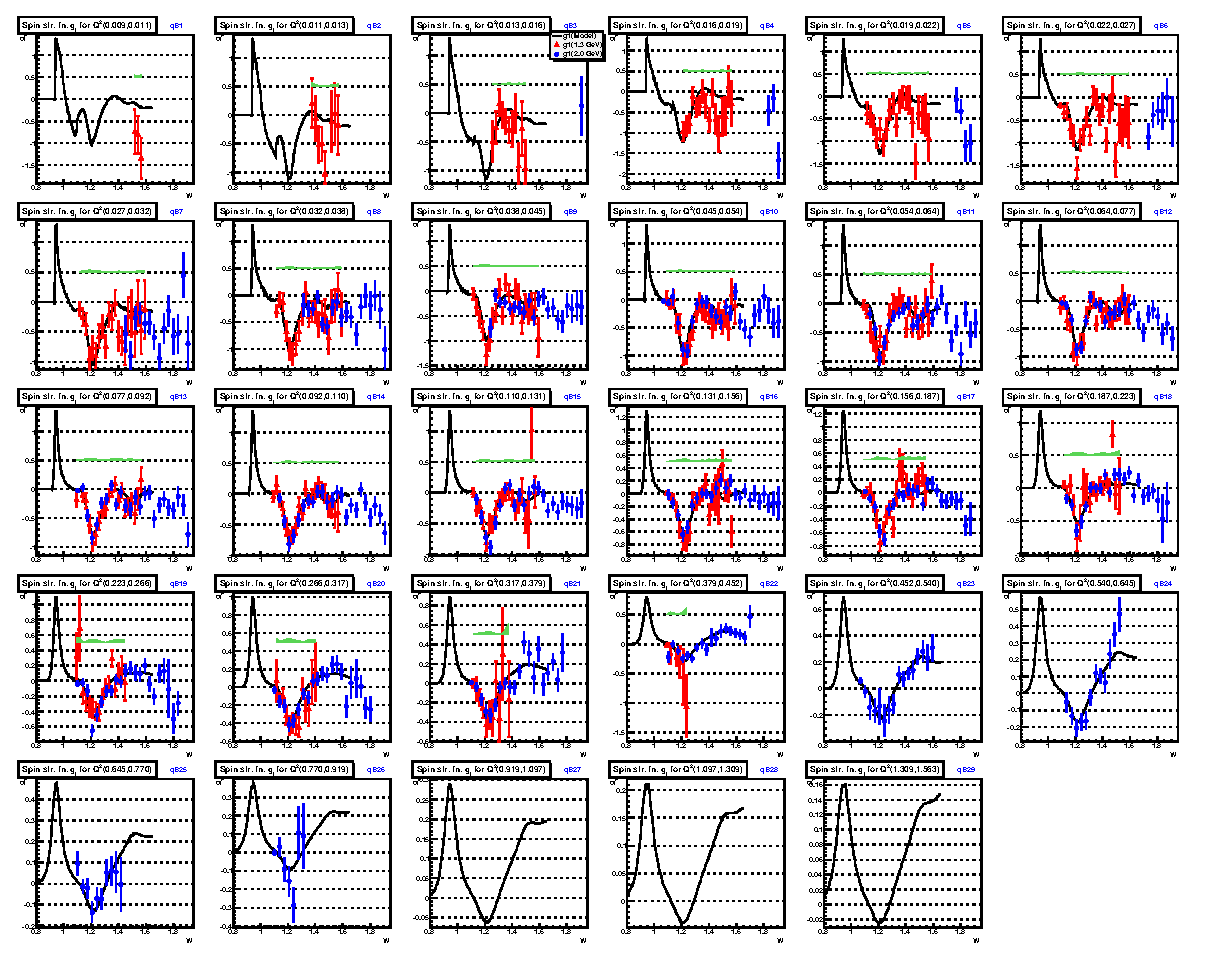
\includegraphics[width=1.0\textwidth]{chap4simul/FigAnal/g1_stdAndExtracted_C194S139EbBothNoQe.eps} 
  %\leavevmode 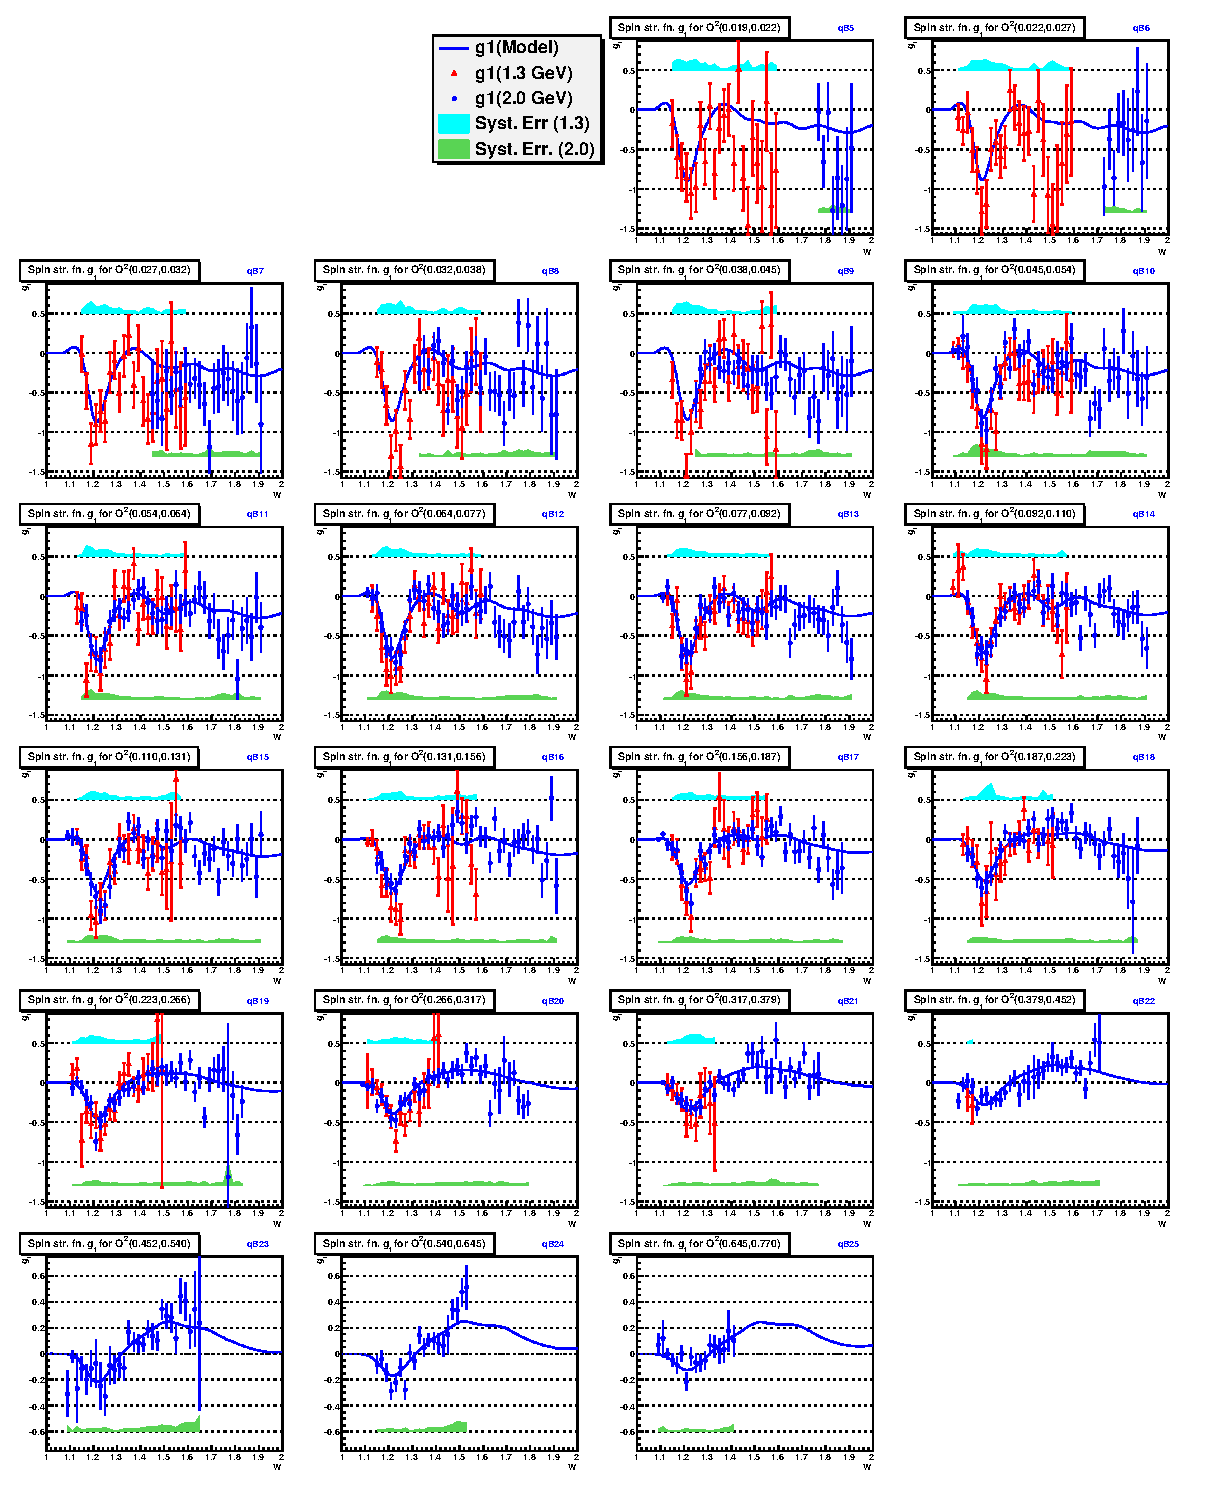
\includegraphics[width=1.0\textwidth]{chap4simul/FigAnal/extractedFrmBothEb_G1_C194S139NoQeWbins70LessQ2bins.eps} 
  %\leavevmode 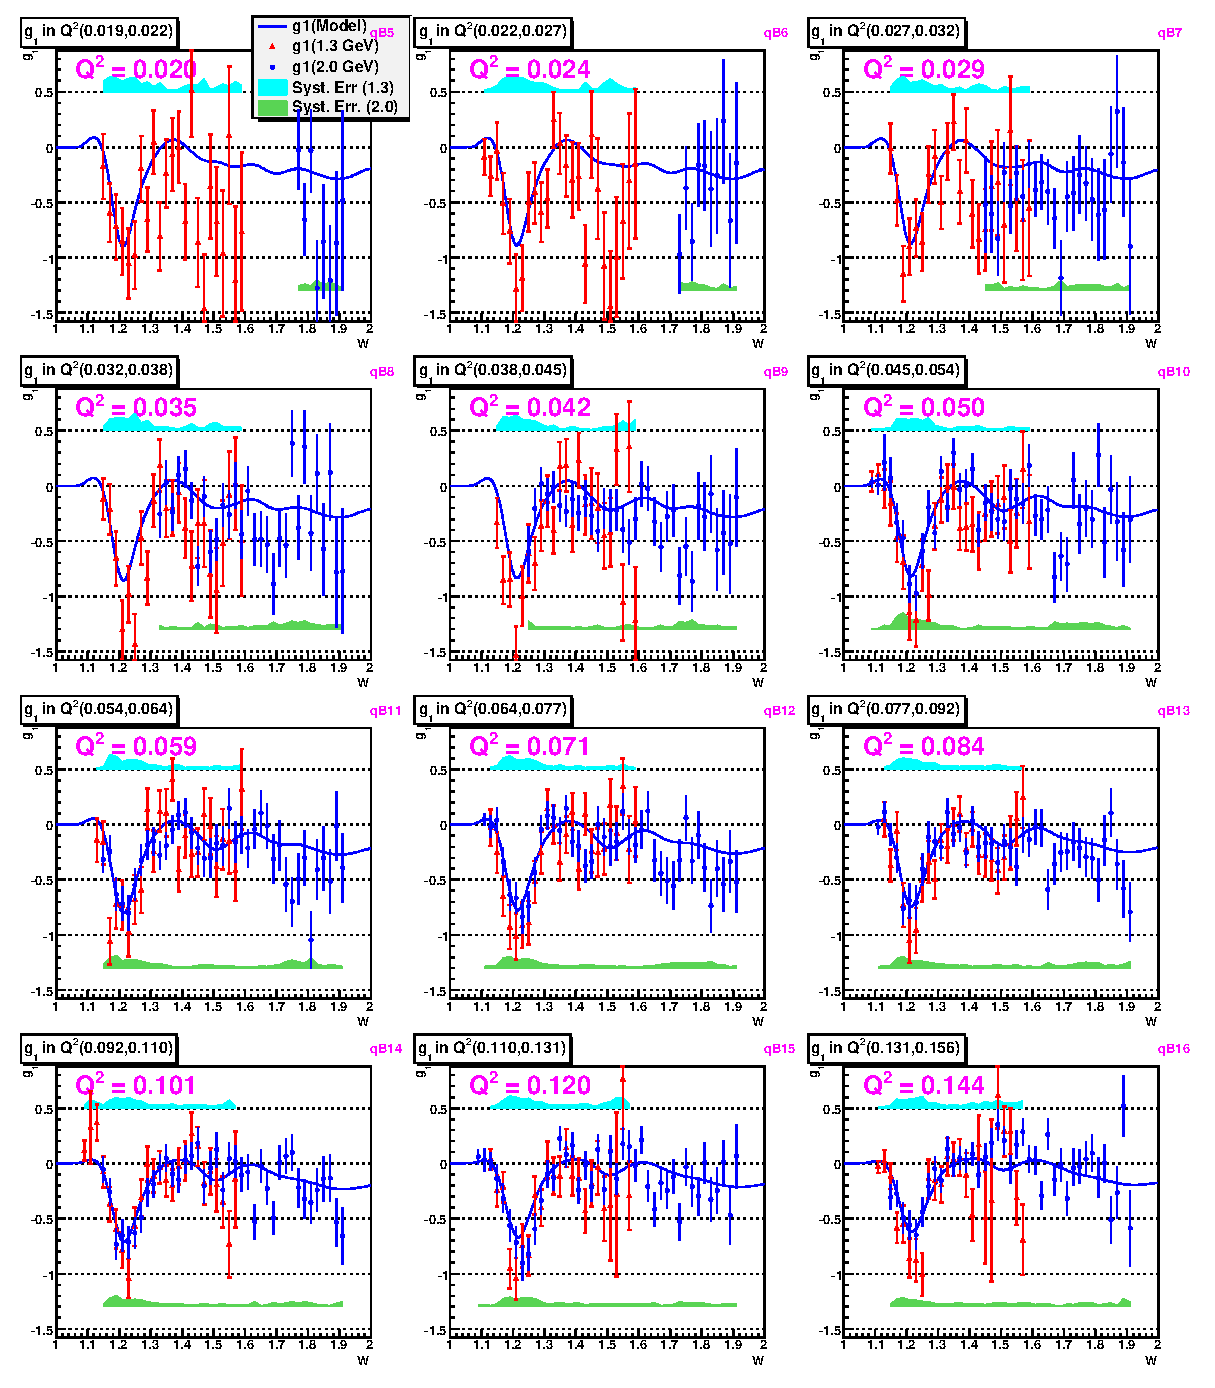
\includegraphics[width=1.0\textwidth]{chap4simul/FigAnal/extractedFrmBothEb_G1_C194S139NoQeWbins70LessQ2binsNwPd.eps} 
  \leavevmode 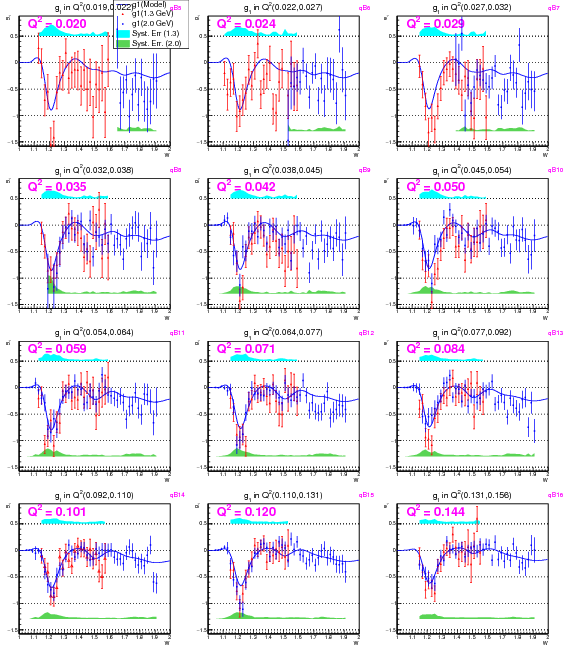
\includegraphics[width=1.0\textwidth]{figuresEG4/FigResults/extractedFrmBothEb_G1_C71S181NoQeWbins70LessQ2binsNwPd.png} 
  \caption[Extracted $g_{1}$ in the first 12 \qsqs bins]{Extracted $g_{1}$ for deuteron (in the first 12 \qsqs bins) from the two different beam energy data sets. The statistical errors are indicated by error bars, while the systematic uncertainties are given by the bands (\textcolor{cyan}{cyan}, top: 1.3 GeV and \textcolor{green}{green}, bottom: 2 GeV).}
  \label{extG1}  %http://wwwold.jlab.org/Hall-B//secure/eg4/adhikari/Analysis/SimStuffs/Extracted_g1/ResIfarm0901/NewRes/
\end{figure}

\begin{figure}[H] %[ht] %ht, htpb (p - float, b = bottom, h=? t = top)
%  \leavevmode 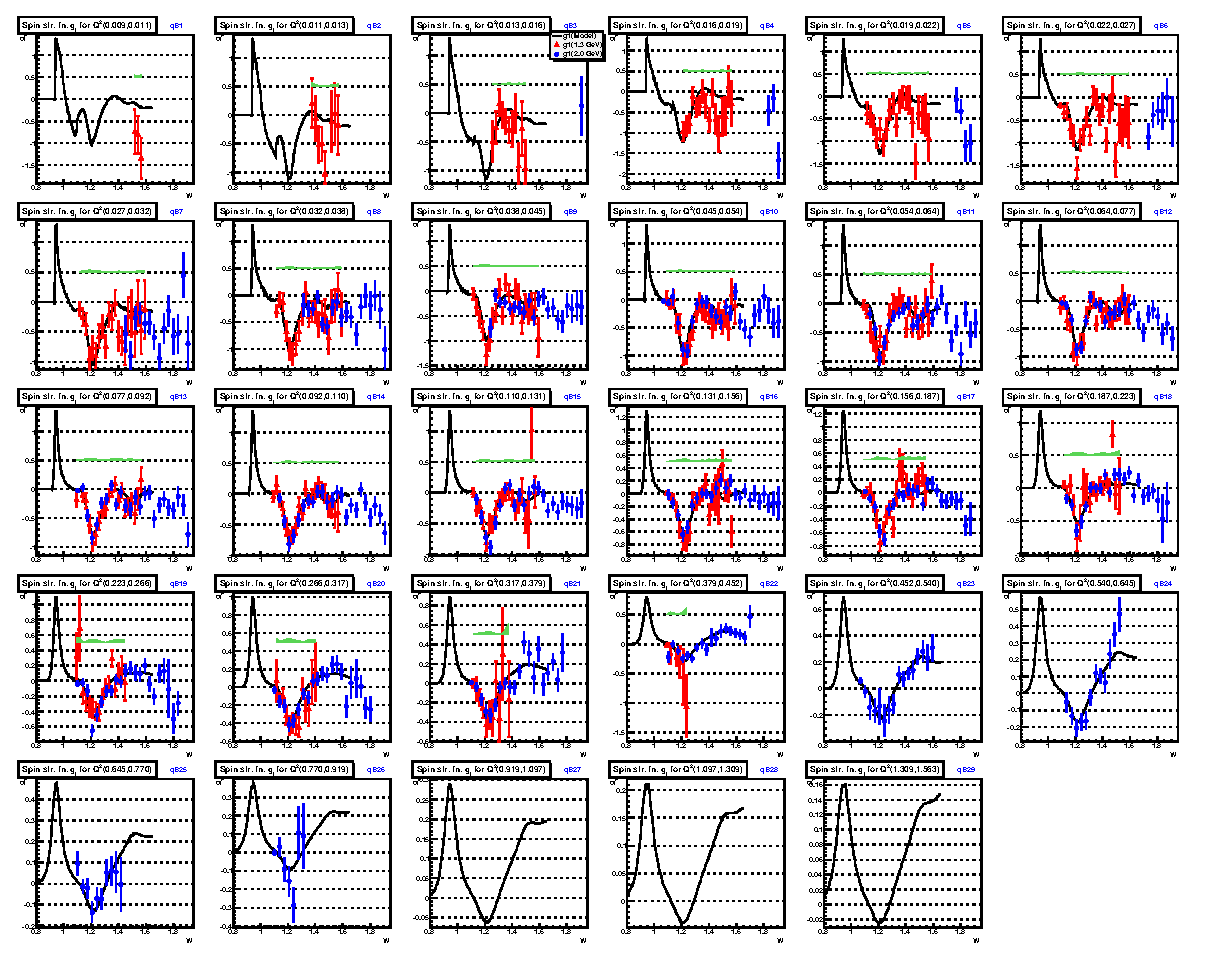
\includegraphics[width=1.0\textwidth]{chap4simul/FigAnal/g1_stdAndExtracted_C194S139EbBothNoQe.eps} 
  %\leavevmode 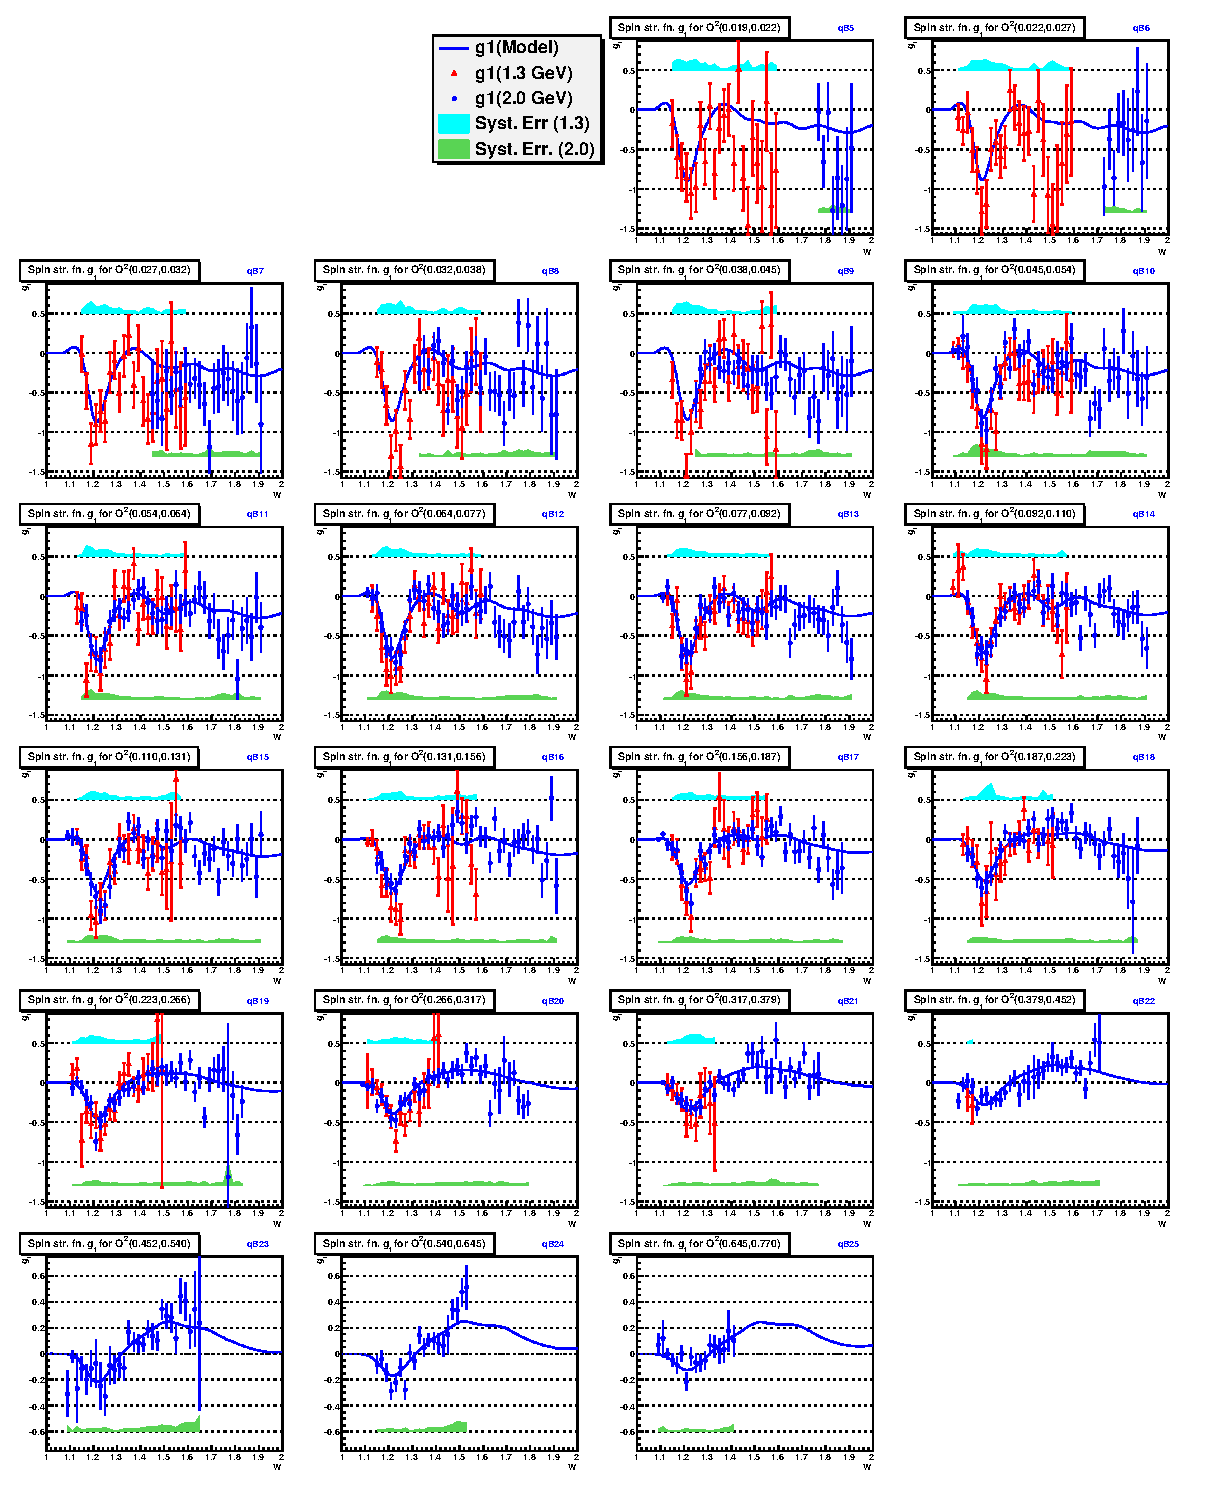
\includegraphics[width=1.0\textwidth]{chap4simul/FigAnal/extractedFrmBothEb_G1_C194S139NoQeWbins70LessQ2bins.eps} 
  %\leavevmode 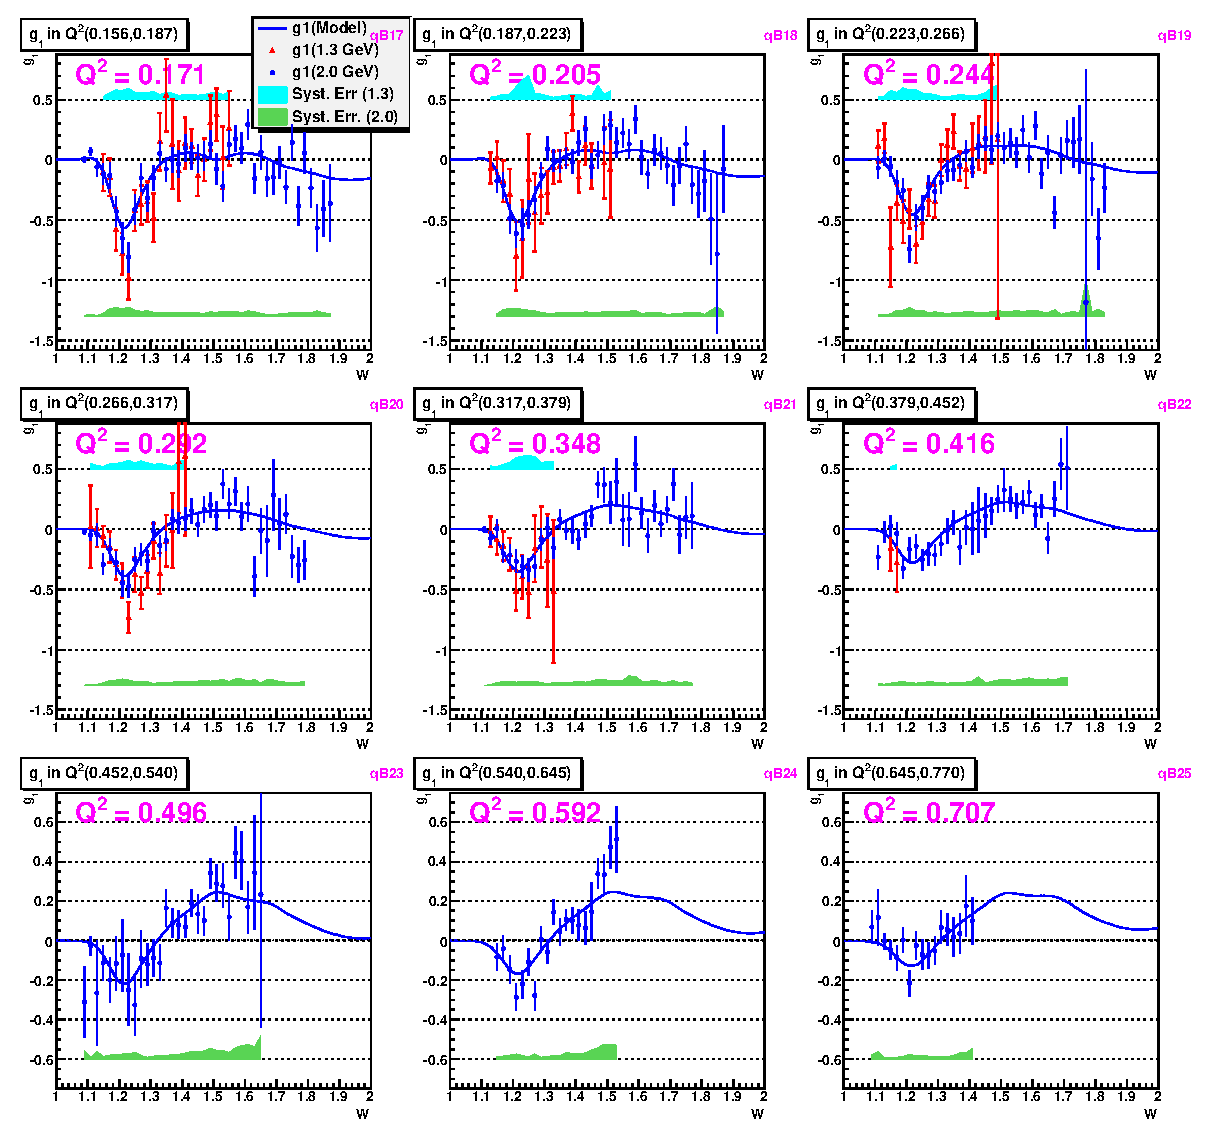
\includegraphics[width=1.0\textwidth]{chap4simul/FigAnal/extractedFrmBothEb_G1_C194S139NoQeWbins70LessQ2binsNwPd3.eps} 
  \leavevmode 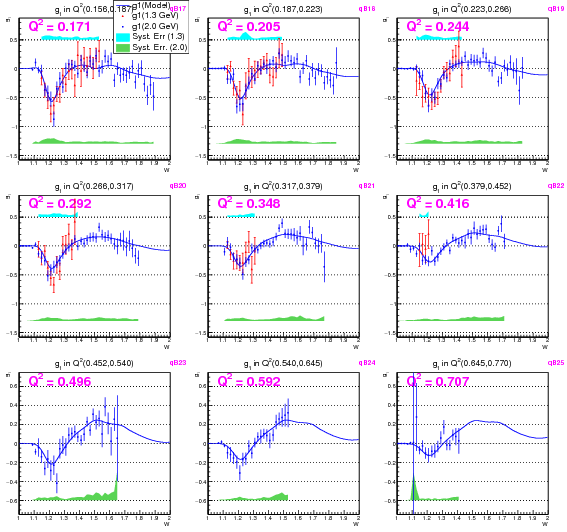
\includegraphics[width=1.0\textwidth]{figuresEG4/FigResults/extractedFrmBothEb_G1_C71S181NoQeWbins70LessQ2binsNwPd3.png} 
  \caption[Extracted $g_{1}$ in the next 9 \qsqs bins]{Extracted $g_{1}$ for deuteron (in the last 9 \qsqs bins (see Fig. \ref{extG1} for the first 12 bins)) from the two different beam energy data sets.}
  \label{extG13}  %http://wwwold.jlab.org/Hall-B//secure/eg4/adhikari/Analysis/SimStuffs/Extracted_g1/ResIfarm0901/NewRes/
\end{figure}

%\end{comment}

Likewise, Figs. \ref{extA1F14} and \ref{extA1F13} shows the extracted values of \afones and their errors from two different beam energies (~1.3 GeV and ~2.0 GeV). %with one overalyed on top of another. 
These values also show similar behavior as \gone. %just as in \gone.
%\begin{comment}

\begin{figure}[H] %[ht] %ht, htpb (p - float, b = bottom, h=? t = top)
  %\leavevmode 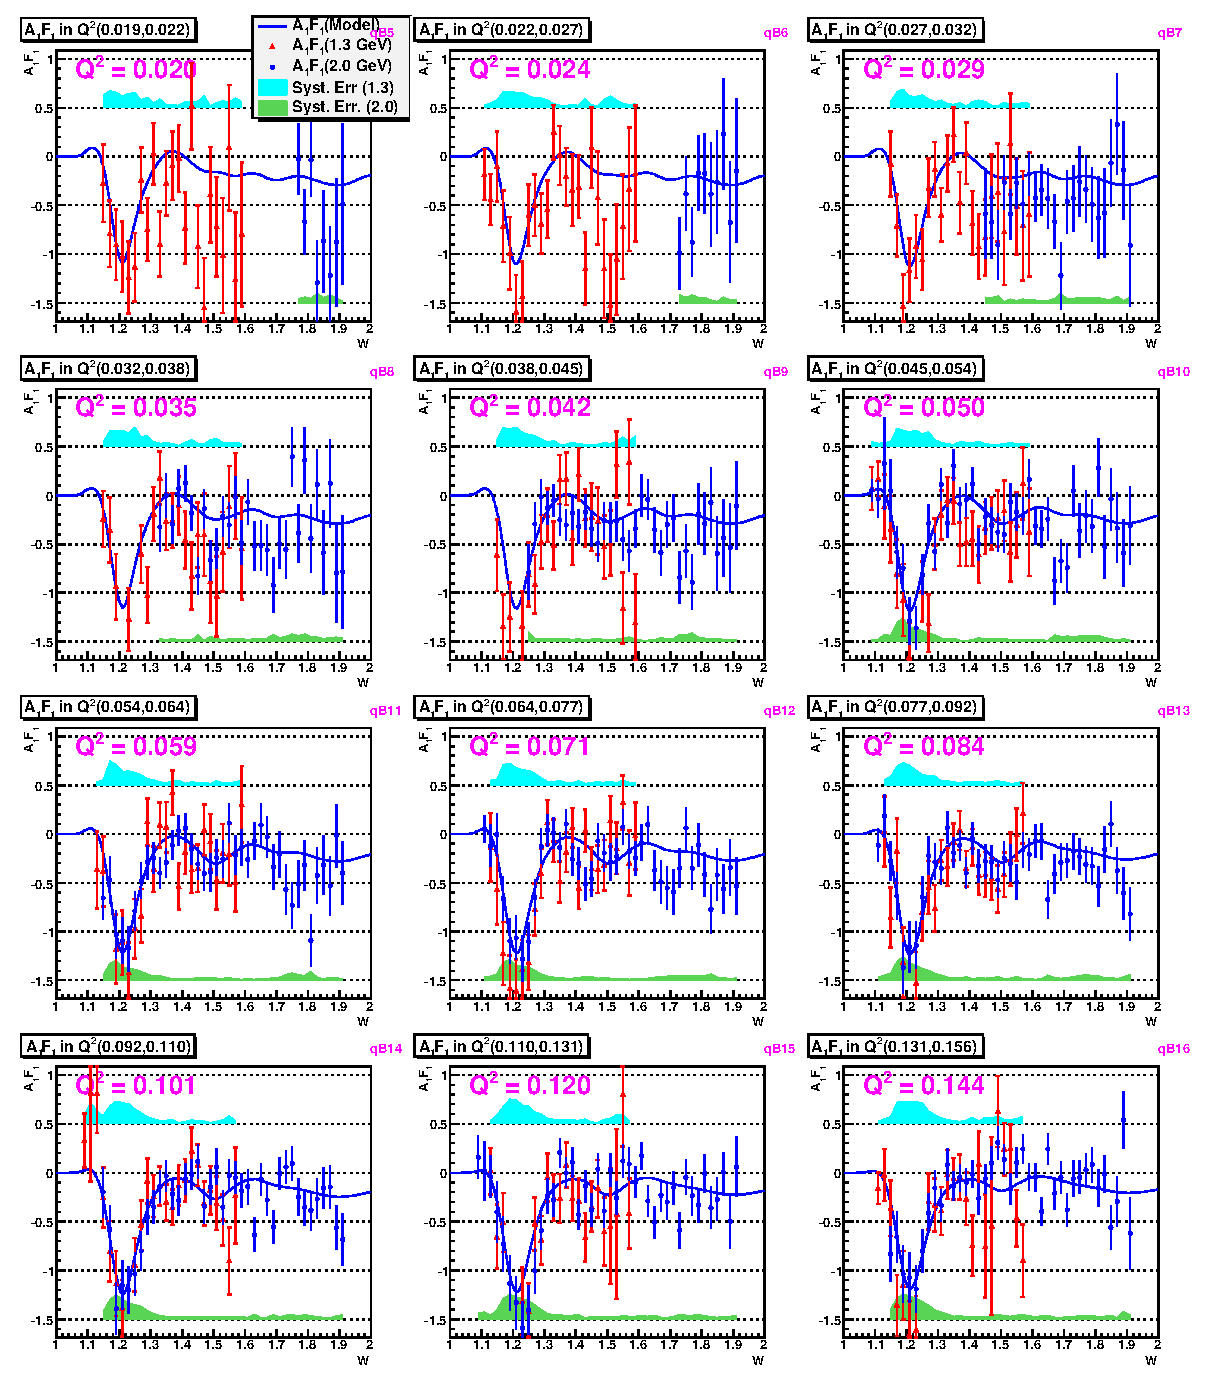
\includegraphics[width=1.0\textwidth]{chap4simul/FigAnal/extractedFrmBothEb_A1F1_C194S139NoQeWbins70LessQ2binsNwPd.eps} 
  \leavevmode 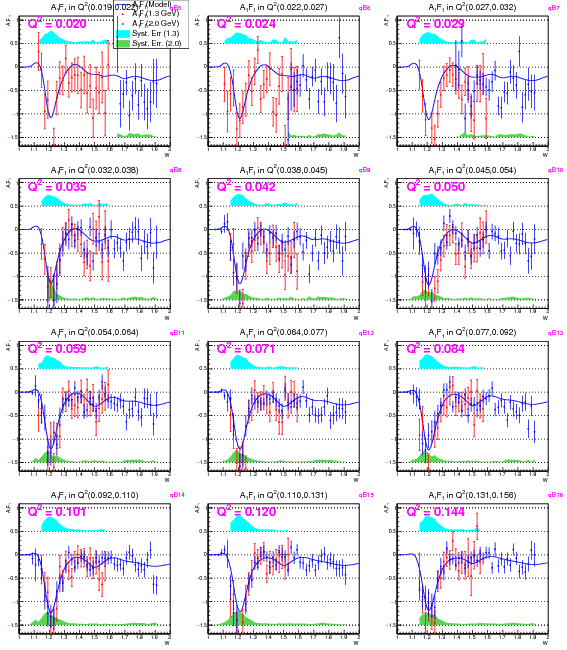
\includegraphics[width=1.0\textwidth]{figuresEG4/FigResults/extractedFrmBothEb_A1F1_C71S181NoQeWbins70LessQ2binsNwPd.png} 
  %\caption[Extracted $A_1 F_1$ in the first 12 \qsqs bins]{Extracted $A_1 F_1$ for deuteron in the first 12 \qsqs bins from the two different beam energy data sets.}
  \caption[Extracted $A_1 F_1$ in the first 12 \qsqs bins]{Extracted $A_1 F_1$ for deuteron (in the first 12 \qsqs bins) from the two different beam energy data sets. The statistical errors are indicated by error bars, while the systematic uncertainties are given by the bands (\textcolor{cyan}{cyan}, top: 1.3 GeV and \textcolor{green}{green}, bottom: 2 GeV).}
  \label{extA1F14}  
\end{figure}

\begin{figure}[H] %[ht] %ht, htpb (p - float, b = bottom, h=? t = top)
  \leavevmode 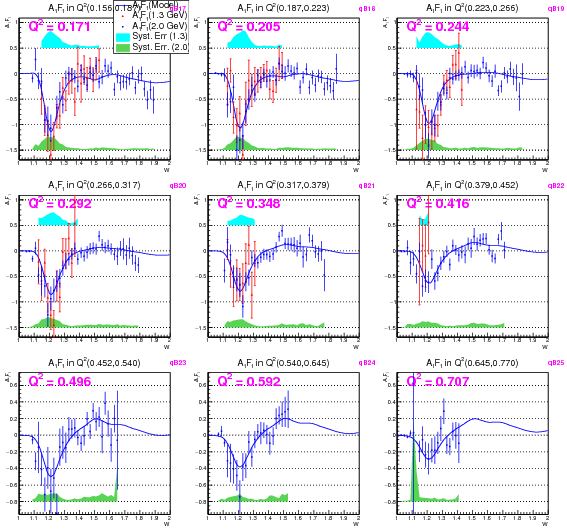
\includegraphics[width=1.0\textwidth]{figuresEG4/FigResults/extractedFrmBothEb_A1F1_C71S181NoQeWbins70LessQ2binsNwPd3.png} 
  \caption[Extracted $A_1 F_1$ in the next 9 \qsqs bins]{Extracted $A_1 F_1$ for for deuteron (in the last 9 \qsqs bins (see Fig. \ref{extA1F14} for the first 12 bins)) from the two different beam energy data sets..}
  \label{extA1F13}  
\end{figure}










Figs. \ref{extG1comb4}, \ref{extG1comb3}, \ref{extA1F1comb4} and \ref{extA1F1comb3} show the values of \gone and \afone and their errors after combining the corresponding results %(bin by bin properly weighing them with their corresponding errors, as described in the previous chapter %\textcolor{red}{ Sec. ref)} 
from the two different beam energies as described in the previous chapter. 


\begin{figure}[H] %[ht] %ht, htpb (p - float, b = bottom, h=? t = top)
  \centering
  \leavevmode 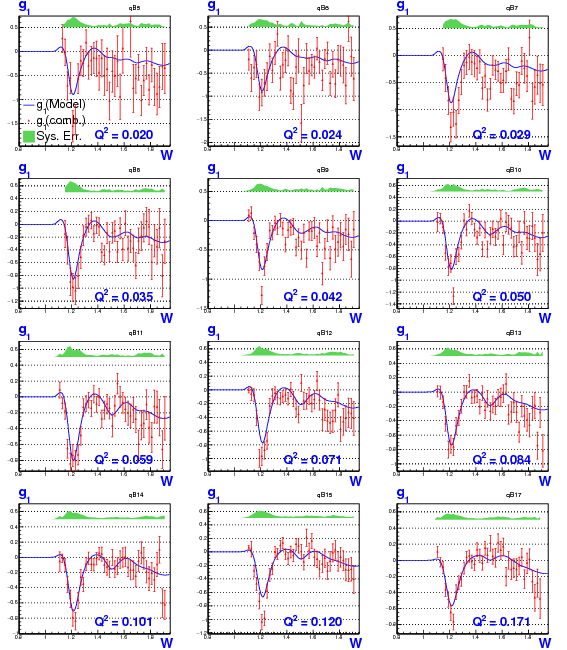
\includegraphics[width=1.0\textwidth]{figuresEG4/FigResults/combinedG1_C71S181EbBothNoQeWbins70NwPd.png} 
  \caption[Combined $g_{1}$ (in first 12 \qsqs bins)]{Extracted $g_{1}$ for deuteron after combining the results from the two beam energies (in the first 12 \qsqs bins). The red data points with error bars in each of the panels are the combined extracted results, the blue continuous line is the used model of \gones and the green band represents the corresponding total systematic errors.}
  \label{extG1comb4} 
\end{figure}

\begin{figure}[H] %[ht] %ht, htpb (p - float, b = bottom, h=? t = top)
  \centering
  \leavevmode 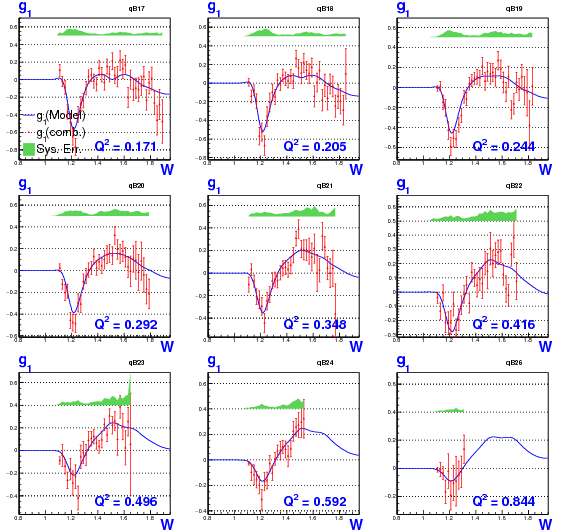
\includegraphics[width=1.0\textwidth]{figuresEG4/FigResults/combinedG1_C71S181EbBothNoQeWbins70NwPd3.png} 
  \caption[Combined $g_{1}$ (in next 9 \qsqs bins)]{Similar plots as in Fig. \ref{extG1comb4} showing the combined results on \gones in the next 9 \qsqs bins.}
  \label{extG1comb3} 
\end{figure}



\begin{figure}[H] %[ht] %ht, htpb (p - float, b = bottom, h=? t = top)
  \centering
  \leavevmode 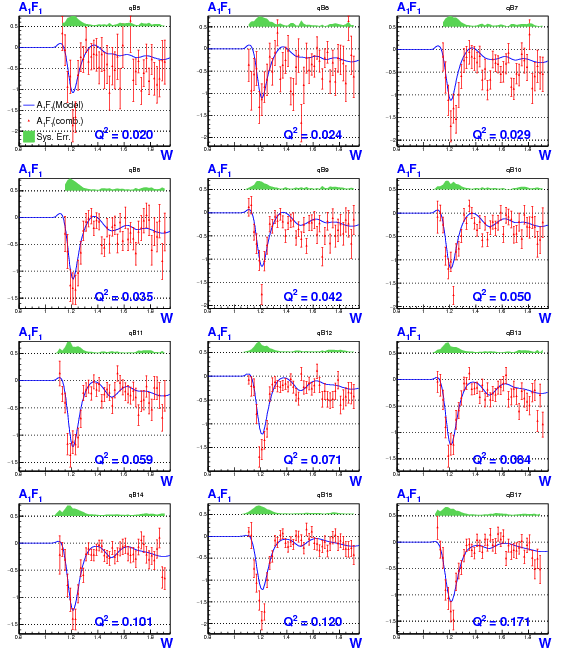
\includegraphics[width=1.0\textwidth]{figuresEG4/FigResults/combinedA1F1_C71S181EbBothNoQeWbins70NwPd.png} 
  \caption[Combined $A_1 F_1$ (in first 12 \qsqs bins)]{$A_1 F_1$ after combining the results from the two beam energies (in the first 12 \qsqs bins). The red data points with error bars in each of the panels are the combined extracted results, the blue continuous line is the used model of \gones and the green band represents the corresponding total systematic errors.}
  \label{extA1F1comb4}  
\end{figure}

\begin{figure}[H] %[ht] %ht, htpb (p - float, b = bottom, h=? t = top)
  \centering
  \leavevmode 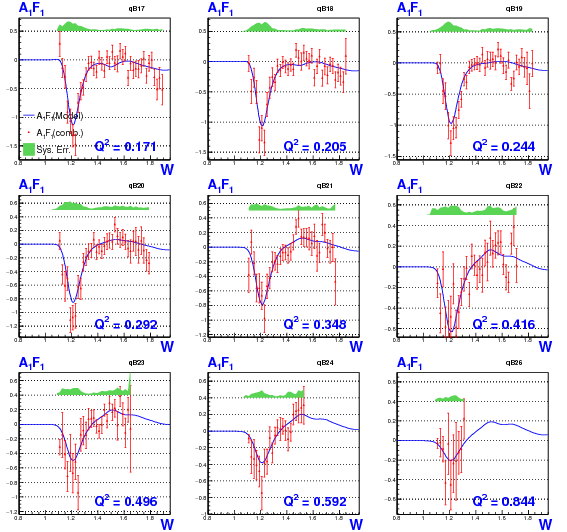
\includegraphics[width=1.0\textwidth]{figuresEG4/FigResults/combinedA1F1_C71S181EbBothNoQeWbins70NwPd3.png} 
  \caption[Combined $A_1 F_1$ (in next 9 \qsqs bins)]{Similar plots as in Fig. \ref{extA1F1comb4} showing the combined results on \gones in the next 9 \qsqs bins.}
  \label{extA1F1comb3}  
\end{figure}




\begin{comment}
\section{Systematic Errors in the Extracted \gones, \afones}
The figures \ref{extG1SEcomb} and \ref{extA1F1SEcomb} show the breakdown of the total contribution to the systematic error from different sources. We can see that the dominant contribution comes from the uncertainties in the overall scale factor (the cyan band indicated with SF-err in the legend) which is used to normalize the simulated data to make them comparable with data. This uncertainty comes mainly from those in $P_bP_t$ and target size measurements. Next big contributions seem to come from the model and radiative corrections. Near the $\Delta$-resonance region, the effect of beam energy uncertainty also seems to be very pronounced. 
%Showing only systematic errors (breakdonw of the 10 components for the beam-energy-combined data)
The breakdown of the different components (but combined between the two beam energies) of the total systematic errors are also shown separately in the figures \ref{extG1SEcomb} and \ref{extA1F1SEcomb}
\begin{figure}[ht] %ht, htpb (p - float, b = bottom, h=? t = top)
  \leavevmode 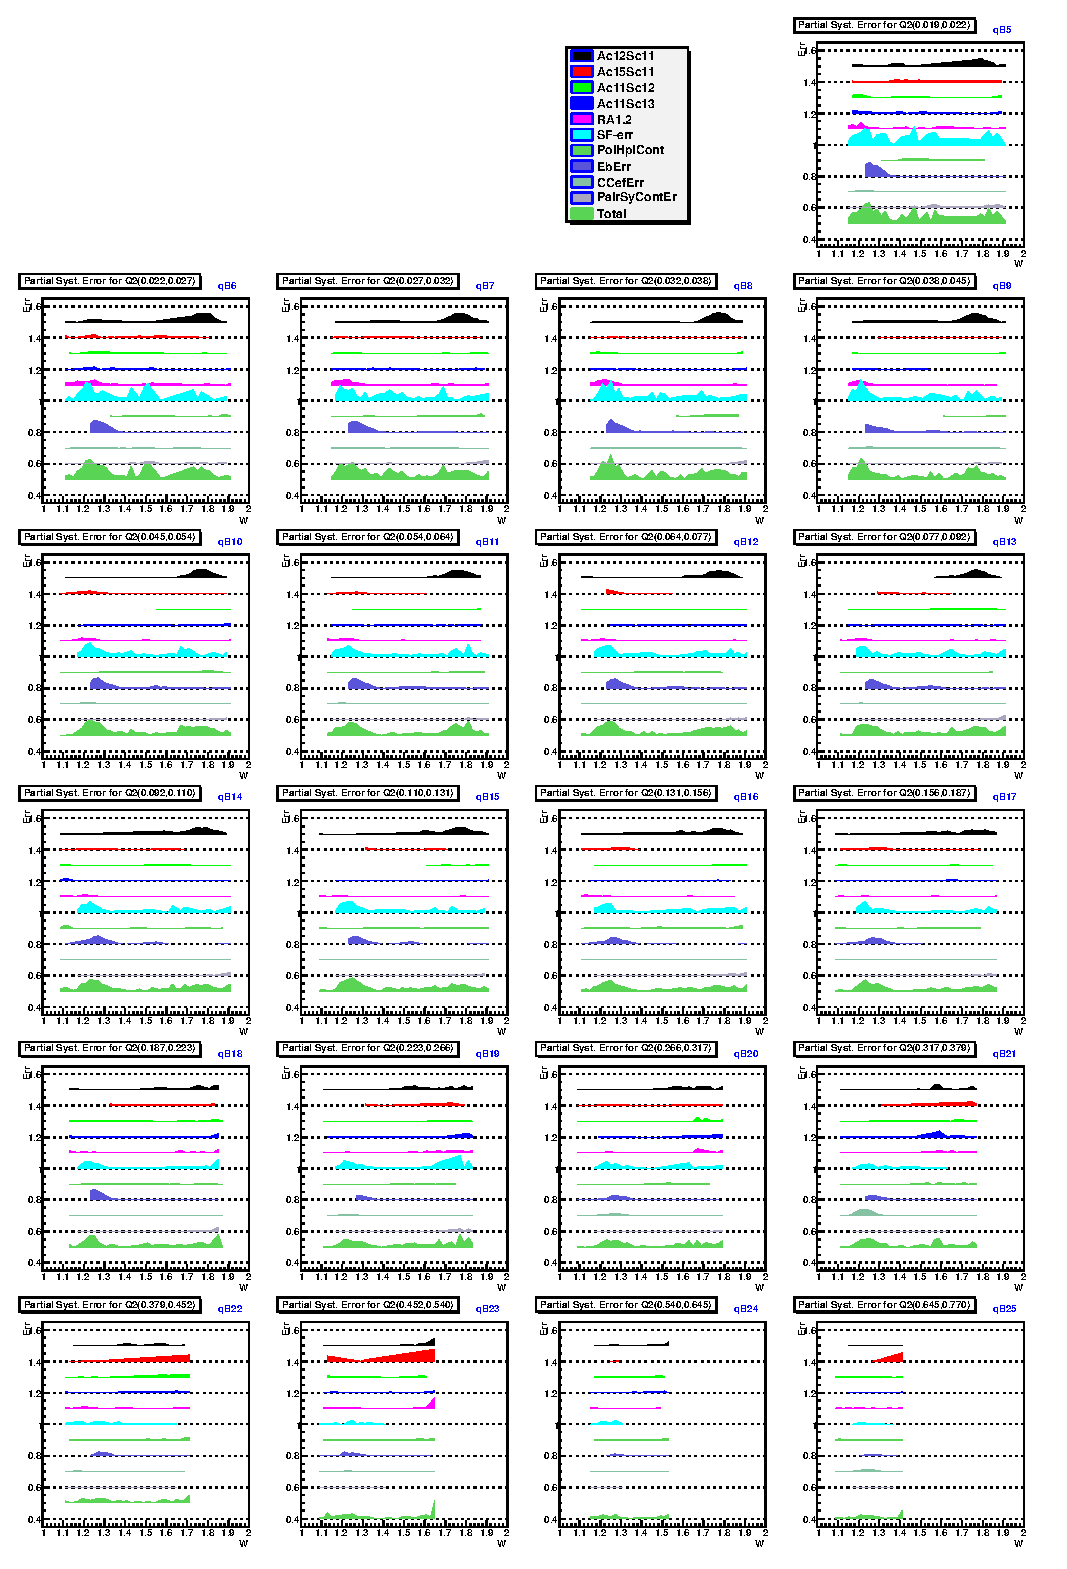
\includegraphics[width=0.95\textwidth]{Chap5Results/Figures/indvSystErrsG1_Eb78Wbins70.eps} 
  \caption[Combined systematic errors in $g_{1}$]{Breakdown of systematic errors in $g_{1}$ (two energy data combined).}
  \label{extG1SEcomb} 
\end{figure}

\begin{figure}[ht] %ht, htpb (p - float, b = bottom, h=? t = top)
  \leavevmode 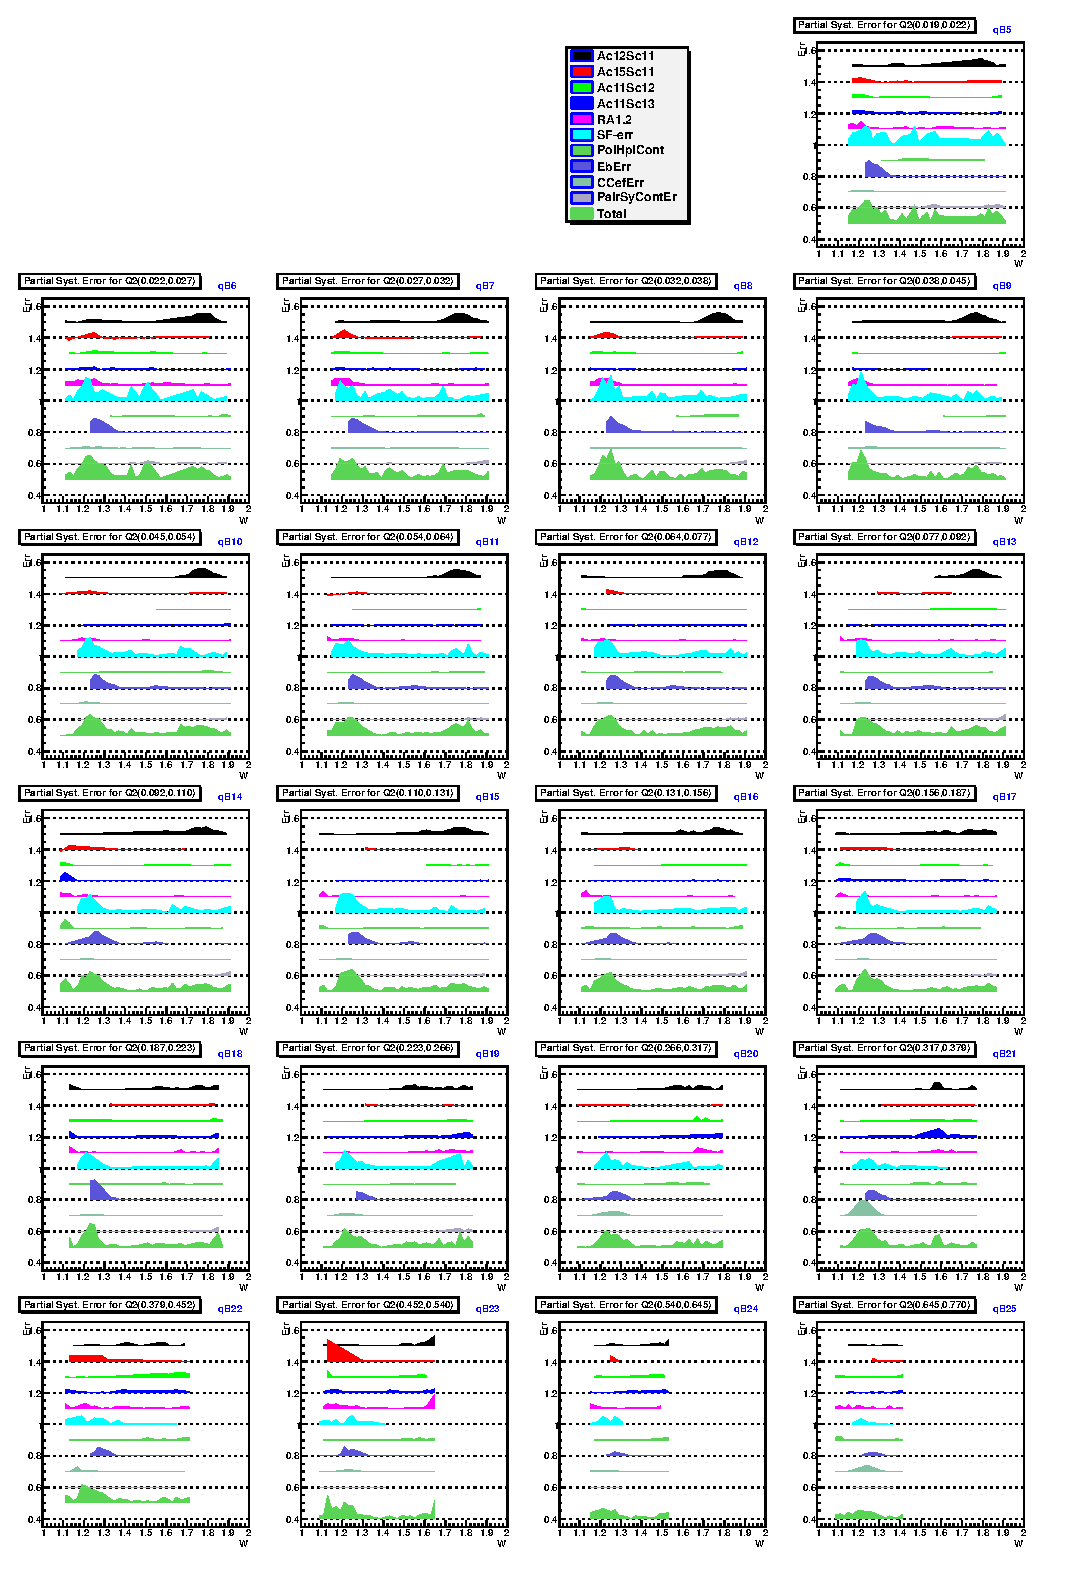
\includegraphics[width=0.95\textwidth]{Chap5Results/Figures/indvSystErrsA1F1_Eb78Wbins70.eps} 
  \caption[Combined systematic errors in $A_1 F_1$]{Breakdown of systematic errors in $A_1 F_1$ (two energy data combined).}
  \label{extA1F1SEcomb}  
\end{figure}
\end{comment}



%\section{Some Integrals measured for the Deuteron target} %SEK
\section{Moments of Deuteron Spin Structure functions}
Using the measured values of \gones and \afone, three integrals were evaluated for each of the \qsqs bins in which these data were measured. These integrals have been calculated in two ways - using only the new EG4 measurements, and adding model contributions to the data %previous one 
for regions not covered by our measurements. %where the measurements were not made. 
The integrals with the model contributions were calculated from $x=0.001$ to the onset of the resonance region (i.e. to the pion production threshold of $W\approx 1.08 $ GeV), dividing the sum into three parts for each \qsqs bin. For example, $\Gamma_1$ was evaluated by adding up the product $g_1 \Delta x$ over the following three kinematic regions:
\begin{eqnarray}
\label{eqGamma10}
\Gamma_1(Q^2) &=& \int^{x(W_{data})}_{x=0.001}  g_1(x,Q^2) dx \qquad \text{model} \\ % with } \Delta x (\Delta W = 10.0 \text{ MeV}) \\
\label{eqGamma11}
              &+& \int_{x(W_{data})}^{W=1.15}   g_1(x,Q^2) dx \qquad \text{data (or model for gaps)} \\% with } \Delta x (\Delta W = 20.0 \text{ MeV}) \\ 
\label{eqGamma12}
              &+& \int^{W=1.08}_{W=1.15}        g_1(x,Q^2) dx \qquad \text{model} % with} \Delta x (\Delta W = 10.0 \text{1 MeV}) 
\end{eqnarray}
where $W_{data}$ indicates the upper edge of the last $W$ bin in which the EG4 data is available in a given \qsqs bin (the $W$ variable was divided into 70 bins of size 20 MeV in the range W=(0.7,2.1) GeV). The first part of the integral as given by Eq. \ref{eqGamma10} is evaluated by using the model values of \gones and using $\Delta x$ corresponding to a W bin of size 10.0 MeV (The $\Delta W$ is converted to $\Delta x$ by using $x = Q^2/(Q^2 + W^2 - M^2)$ to evaluate $x$ at the two edges of each $W$ bin and taking the difference.). The second part given by Eq. \ref{eqGamma11} is evaluated similarly but using the EG4 results for \gones if there is no measurement gap in between. If there is any gap, the same method as in the first part is used to get a model contribution for the gap and added to the data contribution. Lastly, the the third contribution given by Eq. \ref{eqGamma11} again were evaluated from from model values (quasi-elastic part turned off from the model in all of these cases) but with finer W bins (1 MeV) because the integrals are very sensitive to the region near the $\Delta$ resonance due to the fact that the structure functions show rapid changes in this region. The reason to calculate the third integral using model values rather than data values is to avoid having contributions in the integrals from the quasi-elastic contamination.

The statistical errors are evaluated by adding the statistical error contribution in each $W$ or $x$ bin in quadrature. For example, if the integral is evaluated in a \qsqs bin by calculating the sum $\left( \sum\limits_{W ~bins} g_1 \cdot \Delta x \right) $, then the corresponding statistical error is evaluated by calculating %$\sqrt{ \sum\limits_{W ~bins} g_1 \cdot \Delta x  }$. 
$\sqrt{ \sum\limits_{W ~bins} (\sigma g_1)^2 \cdot \Delta x  }$. %1/6/17: Modified according to Dr. Kuhn's comment (see page 3/98 in ~\Box Sync\KpDocuments\MSUpostdocRelated\EG4\AnalysisNote\EG4_MyOwn\Comments\DrKuhn\Pages96_114Chap7.PDF)
Because the model contribution is assumed to have no statistical uncertainties, the statistical errors in the integrals come solely from the propagation of the statistical error of the measured \gones or \afone.

The other two integrals and their errors are evaluated in the same manner, with \gones replaced by their corresponding integrands and again calculating the three parts of the integrals separately. 

 These integrals are then compared with the latest available predictions from different theories (mainly \chipt) and phenomenological calculations along with EG1b or DIS data whenever applicable.

%\textcolor{red}{I will try my best to put, at least, a little detail on how the integrals were evaluated before the submission tonight} %11/3/13

\subsection{First moment of \gones ($\Gamma_1$)}
The first integral of interest is %we calculated was %SEK
the first moment of \gones i.e., $\Gamma_1$ (see Eq. \ref{eqGamma1}) , which was calculated for all %the 
\qsqs bins for which the new data are %measurements were 
available. Figs. \ref{Gamma1Low} and \ref{Gamma1Log} show the two calculations (with and without model input) along with EG1b data and several \chipts and model predictions. One important observation here is that our measurements provide the only data points in %at %for -SEK, in-GED
the very low \qsqs region (i.e for $Q^2<0.05$ GeV$^2$) where \chipts is thought to be able to make %the only theory that can 
rigorous calculations. Therefore, our data will provide important benchmarks for the future calculations in this kinematics. Particularly, the latest \chipts prediction by Bernard \etal \cite{BEKM13} seems to agree remarkably well in %at %SEK
the very low \qsqs region.

While all other higher \qsqs predictions, except that of Ji \etalns, seem to be within the uncertainties of our measurements, it can be seen that the phenomenological predictions of Soffer \etal compare slightly better with data than others (excluding, of course, the Bernard \etal prediction).



%From A. Deur thesis pg 35:
%The data Phenomenological model prediction
%Soffer and Teryaev: Model constrained by the sum rule value (photon point) and the DIS expectation. The interpretation is done using the BC sum rule. 

%Gamma1
\begin{figure}[H] %[ht] %ht, htpb (p - float, b = bottom, h=? t = top)
  \centering
  %\leavevmode 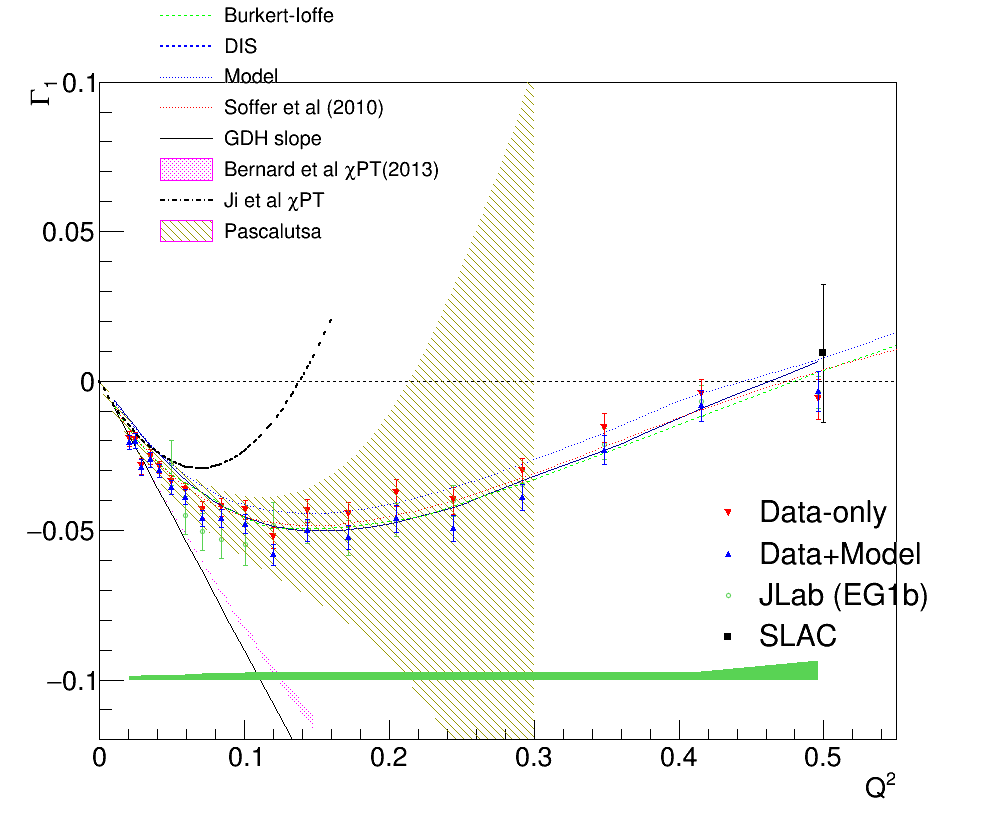
\includegraphics[width=1.0\textwidth]{figuresEG4/FigResults/integralsFromCombinedG1nA1F1_Wbins70Gm1LowQ2.png} 
  \leavevmode 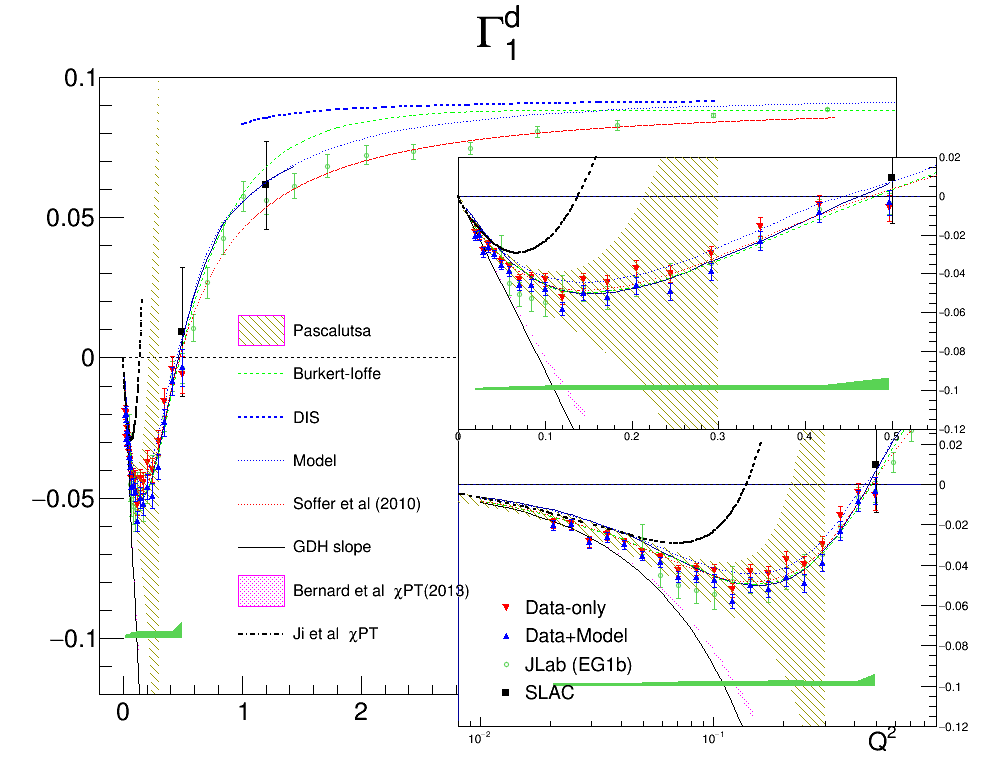
\includegraphics[width=1.2\textwidth]{figuresEG4/FigResults/integralsFromCombinedG1nA1F1_Wbins70Gm1WdInset2.png} 
  \caption[$\Gamma^d_1$ (linear scale).]{Extracted $\Gamma_1$ for deuteron compared with some of the past measurements and various theoretical predictions  with a linear scale used for \qsq. }
  \label{Gamma1Low}  
\end{figure}

\begin{figure}[H] %[ht] %ht, htpb (p - float, b = bottom, h=? t = top)
  \centering
  %\leavevmode 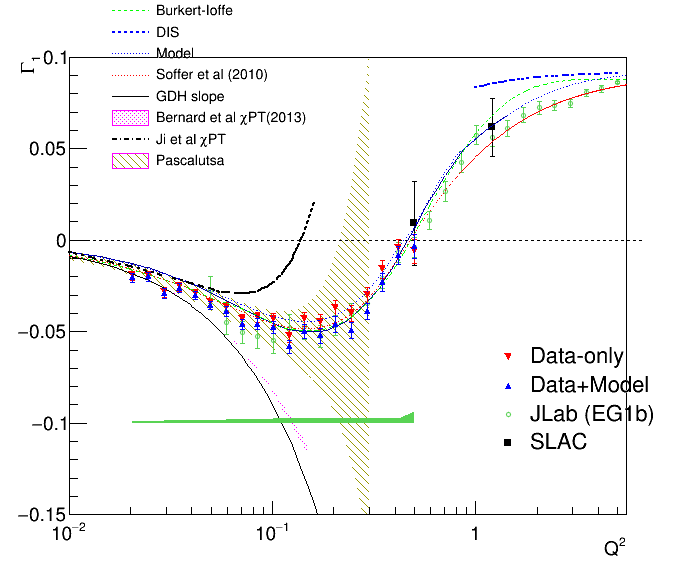
\includegraphics[width=1.0\textwidth]{figuresEG4/FigResults/integralsFromCombinedG1nA1F1_Wbins70Gm1Log.png} 
  \leavevmode 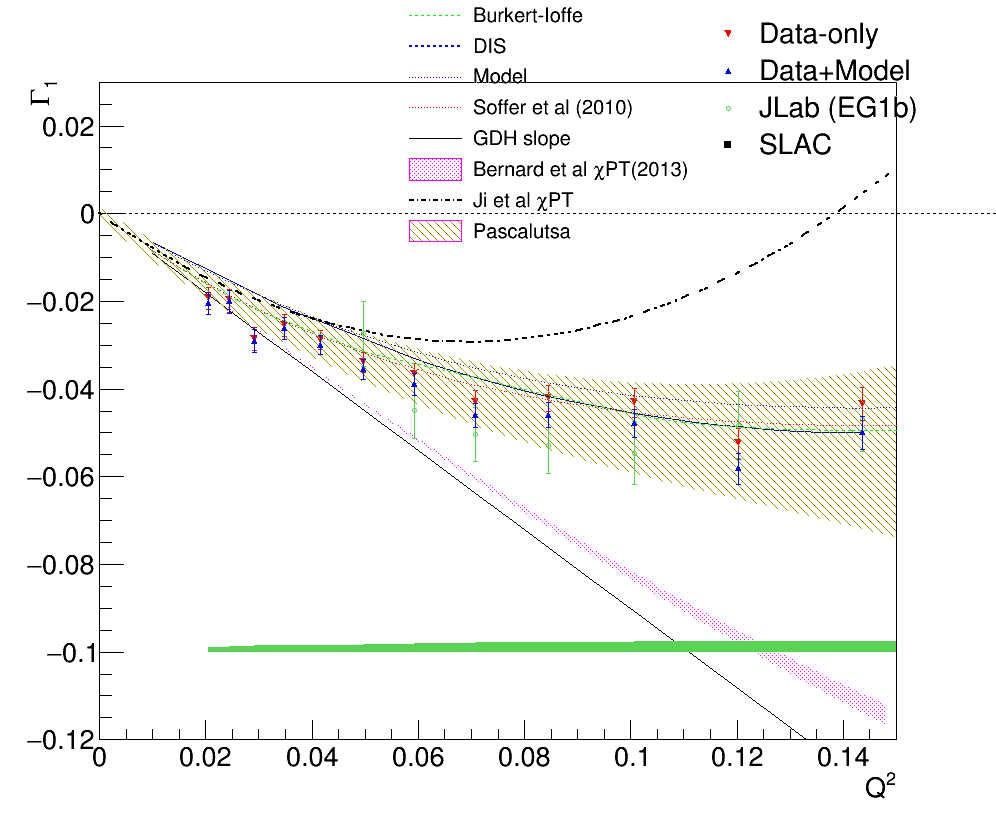
\includegraphics[width=1.0\textwidth]{figuresEG4/FigResults/integralsFromCombinedG1nA1F1_Wbins70Gm1LowerQ2.png} 
  % \caption[$\Gamma^d_1$ (log scale).]{Extracted $\Gamma_1$ for deuteron compared with some of the past measurements and various theoretical predictions  with a logarithmic scale used for \qsq.}
  \caption[$\Gamma^d_1$ (log scale).]{Extracted $\Gamma_1$ for deuteron compared with some of the past measurements and various theoretical predictions zooming in on the very low \qsq region.}
  \label{Gamma1Log}  
\end{figure}






\subsection{The extended GDH integral  $\bar{I}_{TT}$}
Using the %above presented %SEK
measured values of \afone, the generalized GDH integral $\bar{I}_{TT}=2M^2/Q^2 \int A_1F_1(x,Q^2)dx$ was also calculated and compared (see Figs. \ref{GDHLow} and \ref{GDHLog}) with the %on 
latest \chipts calculation from Bernard \etal \cite{BEKM13}. %Again, the prediction and the measurement seem to converse nicely at the very low momentum transfers indicating that their model is in a very good shape in that region but will have to do a lot more to turn their predictions around in the higher \qsqs region.
We can see that at the very low \qsq, the \chipts prediction and the measurement get very close. 
%SEK 11/3/13: Bottom of p. 180: "converse nicely" ??? In fact, that sentence is pretty much meaningless. Instead, what you want to say is the ChPT calculations determine the higher powers of Q^2 in the Taylor expansion of the integrals around the photon point Q^2=0, beyond the prediction of the GDH sum rule which determines the lowest order term. However, only one or two higher order terms can be calculated confidently, since higher orders require additional (unknown) constants. Therefore, ChPT predictions do reasonably well at ultra-low Q^2 but cannot be expected to work at the higher Q^2, where the data show a turn-around and the transition towards positive values.
%Since the
The \chipts methods determine the higher powers of \qsqs in the Taylor expansion of the integral around the photon point $Q^2 = 0$, beyond the prediction of the GDH sum rule which determines the lowest order term. %GED comment: This is not a sentence. I'm not sure what you mean.
Our data seem indeed to converge towards the GDH sum rule at our lowest \qsq. %New SEK line added on 11/28/13 from his comments given on the note on 11/14/13
However, only one or two higher order terms can be calculated confidently, since higher orders require additional (unknown) constants. Therefore, \chipts predictions do reasonably well at ultra-low \qsqs but cannot be expected to work at the higher \qsq, where the data show a turn-around and a %the SEK
transition towards positive values.


%GDH integral
\begin{figure}[H] %[ht] %ht, htpb (p - float, b = bottom, h=? t = top)
  \centering
  \leavevmode 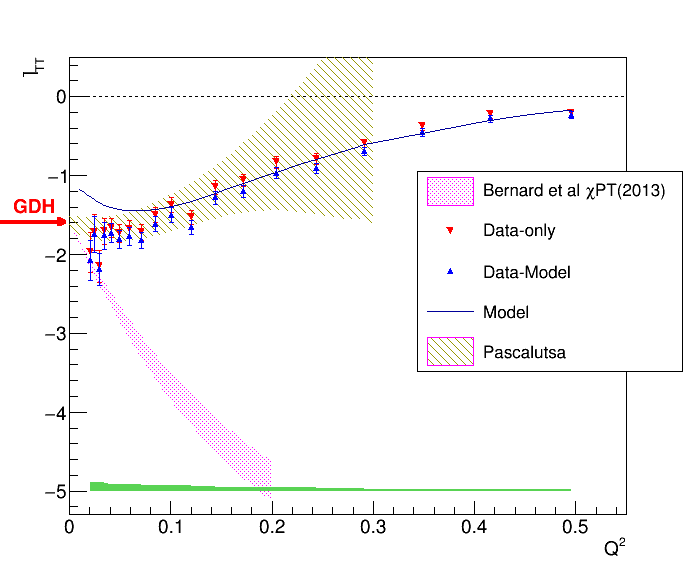
\includegraphics[width=1.0\textwidth]{figuresEG4/FigResults/integralsFromCombinedG1nA1F1_Wbins70IttLowQ2.png} 
  \caption[$\bar{I}_{tt}$ (linear scale)]{Extracted $\bar{I}_{tt}$ for deuteron compared with the used model and a \chipts prediction  with a linear scale used for \qsq.}
  \label{GDHLow}  
\end{figure}

\begin{figure}[H] %[ht] %ht, htpb (p - float, b = bottom, h=? t = top)
  \centering
  \leavevmode 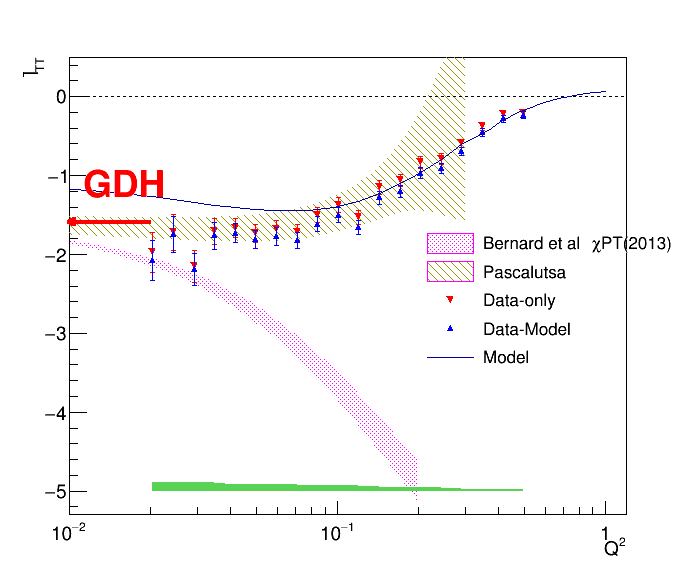
\includegraphics[width=1.0\textwidth]{figuresEG4/FigResults/integralsFromCombinedG1nA1F1_Wbins70IttLogN.png} 
  \caption[$I^d_{tt}$ (log scale)]{Extracted $I_{tt}$ for deuteron compared with the used model and a \chipts prediction  with a logarithmic scale used for \qsq.}
  \label{GDHLog}  
\end{figure}




\subsection{The Generalized Forward Spin Polarizability  $\gamma_0$}
Finally, the generalized forward polarizability (as given by Eq. \ref{polzGm0}) for the deuteron  was also calculated using the measured values of \afones and then compared with various predictions as shown in Figs. \ref{Gamma0Low} and \ref{Gamma0Log}. The comparison shows that both \chipts calculations by Bernard \etal and Kao \etal converge with data at the lowest \qsqs bins. However, the \chipts calculations by Pascalutsa \etal seem to deviate greatly from both the current measurement as well as the other \chipts calculations (particularly at the very low \qsqs region, indicating that some ingredients might be missing from the calculation model.% but MAID prediction seems to be way off the current measurement. %\textcolor{red}{citations?}
Likewise, the MAID prediction also seems to be somewhat off the current results.


%http://tex.stackexchange.com/questions/38524/eps-figures-with-pdflatex using eps with pdflatex
%Gamma1
\begin{figure}[H] %[ht] %ht, htpb (p - float, b = bottom, h=? t = top)
  \centering
  %\leavevmode 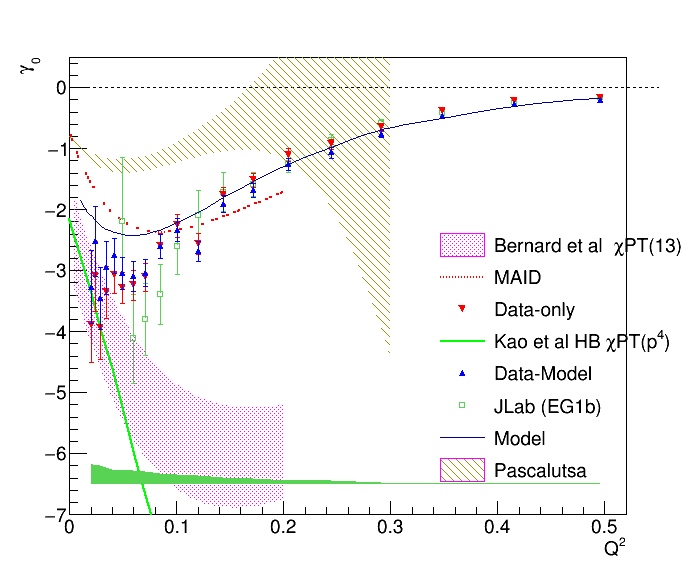
\includegraphics[width=1.0\textwidth]{figuresEG4/FigResults/integralsFromCombinedG1nA1F1_Wbins70Gm0LowQ2.png} 
  \leavevmode 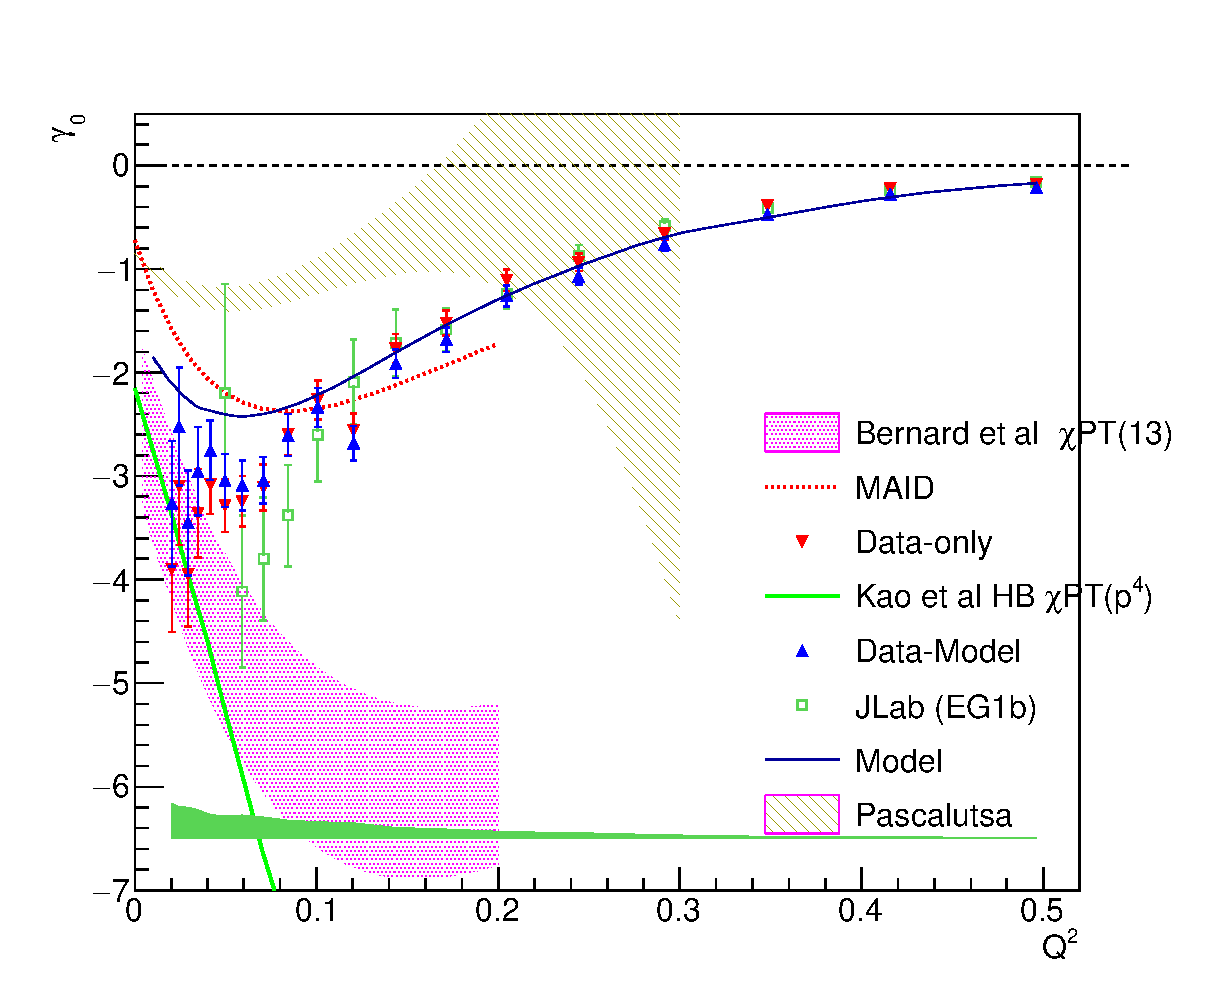
\includegraphics[width=1.0\textwidth]{figuresEG4/FigResults/integralsFromCombinedG1nA1F1_Wbins70Gm0LowQ2} 
  \caption[$\gamma^d_0$ (linear scale)]{Extracted $\gamma_0$ for deuteron compared with some of the past measurements and various theoretical predictions  with a linear scale used for \qsq.}
  \label{Gamma0Low}  
\end{figure}

\begin{figure}[H] %[ht] %ht, htpb (p - float, b = bottom, h=? t = top)
  \centering
  %\leavevmode 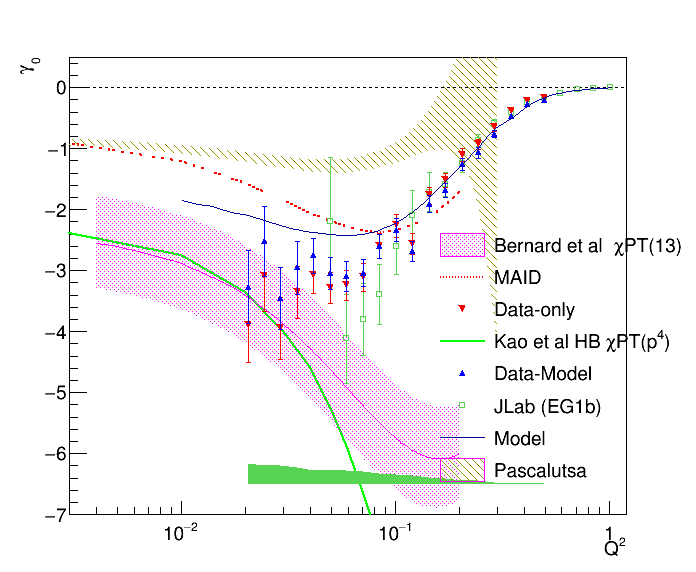
\includegraphics[width=1.0\textwidth]{figuresEG4/FigResults/integralsFromCombinedG1nA1F1_Wbins70Gm0Log.png} 
  \leavevmode 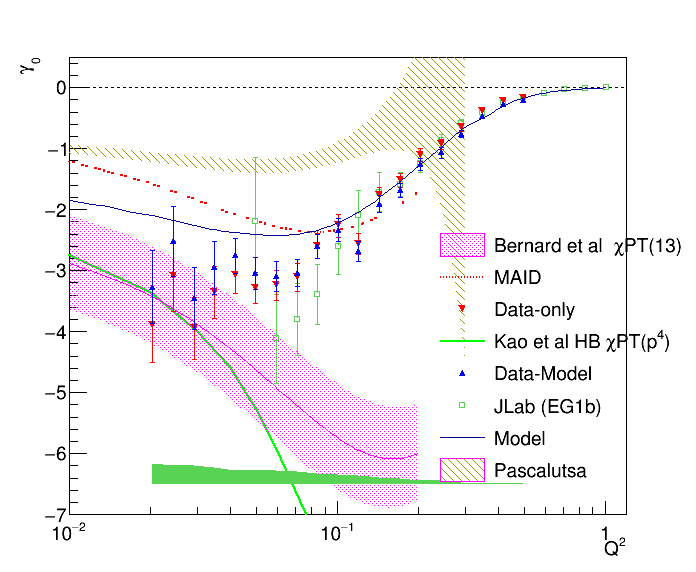
\includegraphics[width=1.0\textwidth]{figuresEG4/FigResults/integralsFromCombinedG1nA1F1_Wbins70Gm0LogN} 
  \caption[$\gamma^d_0$ (log scale)]{Extracted $\gamma_0$ for deuteron compared with some of the past measurements and various theoretical predictions  with a logarithmic scale used for \qsq.}
  \label{Gamma0Log}  
\end{figure}

